\chapter{Design}

This chapter describes the design of the sensor system and all components involved. The system consists of several parts playing different roles. The System Design gives an overview of these parts, their purpose and their communication with each other. Afterwards, these subsystem are described in detail.\\

\section{System Design}

On the user-facing side there is a personal computer (PC). This PC runs software that visualizes a live data stream and provides a control interface for the sensor system. It is connected via USB to a microcontroller. This microcontroller controls the MinieeC interface via I2C, reads the measurement data from it and sends it to the PC. It also controls the matrix switches. The MinieC Interface provides the signal and ground between which the resistance is measured. Both lines are connected to one matrix switch each. These matrix switches are able to connect one input to 8 different outputs. On each of those outputs, one electrode is connected. The matrix switches can thereby connect the MinieC interface to one of 8 electrode pairs. \\

Using the matrix switches, 8 electrodes can be used with just one MinieC interface. Increasing the number of electrodes can be done in two ways:

\begin{itemize}
    \item by chaining up multiple stages of matrix switches, the number of electrodes can be increased eightfold with each stage
    \item by connecting another MinieC Interface with it's own set of matrix switches to the microcontroller, 8 more electrodes can be added with each of these subsystems
\end{itemize}

The first option results in lower cost per added electrode, as the MinieC interface is reused. However, with a system like that, all electrodes have to be read in serial, while with the second option each MinieC interface can read in parallel, resulting in higher sample rate. Practically the second option is also easier to achieve. For the first option, a board with 18 matrix switches and 80 connections is needed, while the second option only uses 2 switches per board resulting in 16 connections. The simpler board greatly reduces complexity and can also be made smaller.

\begin{figure}
	\begin{center}
\begin{tikzpicture}
	\begin{pgfonlayer}{nodelayer}
		\node [rounded corners=8pt, inner sep=16pt, style=rect] (0) at (8, -1) {8 Electrodes};
		\node [rounded corners=8pt, inner sep=16pt, style=rect] (1) at (0, 3) {Microcontroller};
		\node [rounded corners=8pt, inner sep=16pt, style=rect] (2) at (-3, -1) {MinieC Interface};
		\node [rounded corners=8pt, inner sep=16pt, style=rect] (3) at (3, 0.25) {Matrix Switch};
		\node [rounded corners=8pt, inner sep=16pt, style=rect] (4) at (0, 6) {PC};
		\node [style=rect, inner sep=16pt, rounded corners=8pt] (5) at (3, -2.25) {Matrix Switch};
	\end{pgfonlayer}
	\begin{pgfonlayer}{edgelayer}
		\draw [style=darrow] (4) to node[left]{USB} (1);
		\draw [style=simple, bend right=15, looseness=1.00] (0) to node[above]{8 SIG} (3);
		\draw [style=simple, bend right=15, looseness=1.00] (3) to node[above]{SIG} (2);
		\draw [style=arrow, bend left=15, looseness=1.00] (1) to node[right]{SPI} (3);
		\draw [style=darrow, bend right=15, looseness=1.00] (1) to node[left]{I2C} (2);
		\draw [style=simple, bend right=15, looseness=1.00] (2) to node[below]{GND} (5);
		\draw [style=simple, bend right=15, looseness=1.00] (5) to node[below]{8 GND} (0);
		\draw [style=arrow, bend left=15, looseness=1.00] (1) to node[right, pos=0.9]{SPI} (5);
	\end{pgfonlayer}
		\draw (-5.5,-3.5) -- (10,-3.5) -- (10,2) node[below, left, yshift=-8pt] {$n$} -- (-5.5,2) -- (-5.5,-3.5);
\end{tikzpicture}
		%\begin{tikzpicture}
	\begin{pgfonlayer}{nodelayer}
		\node [rounded corners=8pt, inner sep=16pt, style=rect] (0) at (8, -1) {8 Electrodes};
		\node [rounded corners=8pt, inner sep=16pt, style=rect] (1) at (0, 3) {Microcontroller};
		\node [rounded corners=8pt, inner sep=16pt, style=rect] (2) at (-3, -1) {MinieC Interface};
		\node [rounded corners=8pt, inner sep=16pt, style=rect] (3) at (3, 0.25) {Matrix Switch};
		\node [rounded corners=8pt, inner sep=16pt, style=rect] (4) at (0, 6) {PC};
		\node [style=rect, inner sep=16pt, rounded corners=8pt] (5) at (3, -2.25) {Matrix Switch};
	\end{pgfonlayer}
	\begin{pgfonlayer}{edgelayer}
		\draw [style=darrow] (4) to node[left]{USB} (1);
		\draw [style=simple, bend right=15, looseness=1.00] (0) to node[above]{8 SIG} (3);
		\draw [style=simple, bend right=15, looseness=1.00] (3) to node[above]{SIG} (2);
		\draw [style=arrow, bend left=15, looseness=1.00] (1) to node[right]{SPI} (3);
		\draw [style=darrow, bend right=15, looseness=1.00] (1) to node[left]{I2C} (2);
		\draw [style=simple, bend right=15, looseness=1.00] (2) to node[below]{GND} (5);
		\draw [style=simple, bend right=15, looseness=1.00] (5) to node[below]{8 GND} (0);
		\draw [style=arrow, bend left=15, looseness=1.00] (1) to node[right, pos=0.9]{SPI} (5);
	\end{pgfonlayer}
\end{tikzpicture}
		%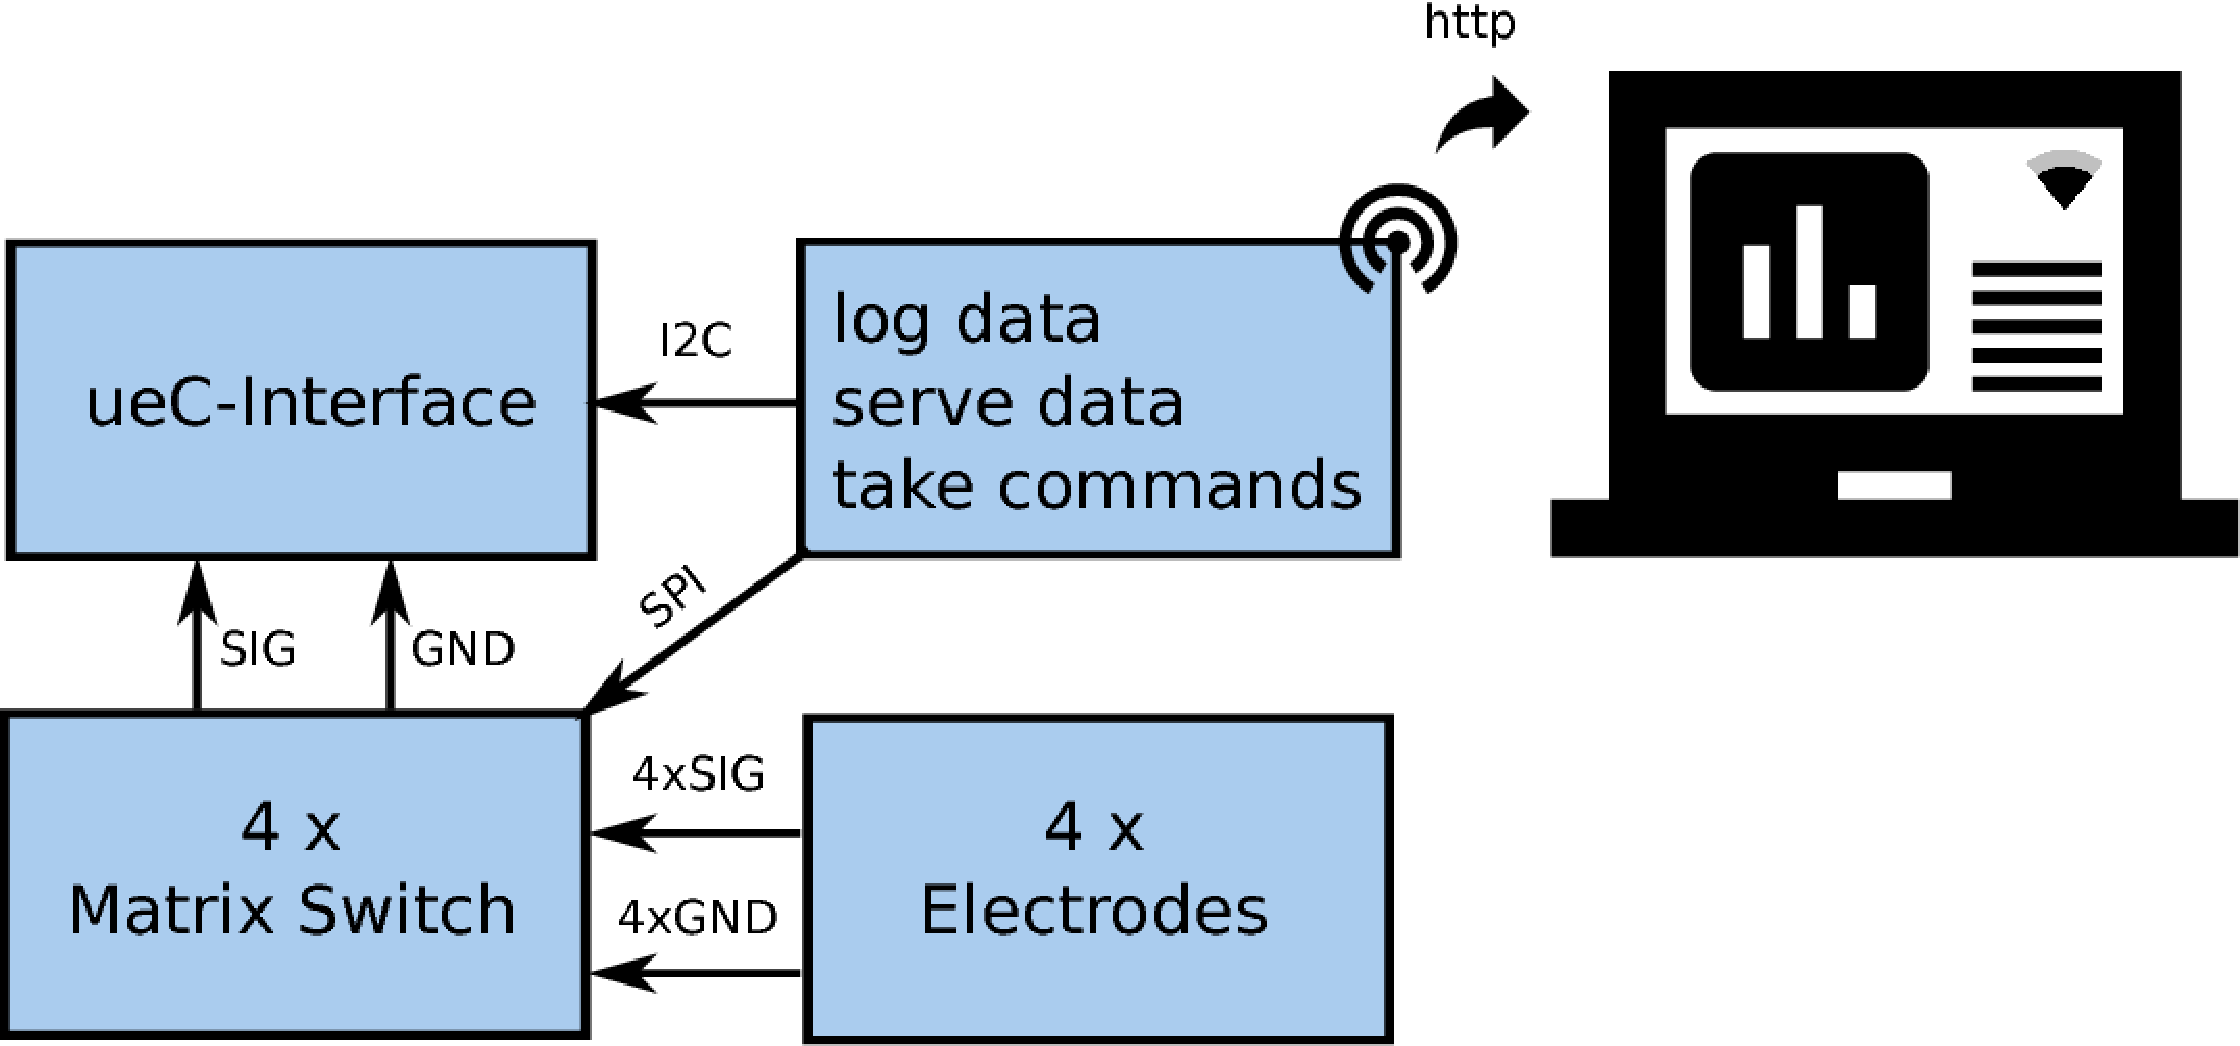
\includegraphics[width=\textwidth]{images/systemdesign.pdf} 
		\caption{System Design}
		\label{fig:sys}
	\end{center}
\end{figure}

\section{Electrodes}

The electrode pairs are the actual sensors in contact with the fluid to be measured. Their material and geometry influence the measuring range of the system. According to information in the book \cite{trankler2015sensortechnik} a cell constant $ C $ of $1$ enables a range from \unitfrac[$2 \cdot 10^3$]{$\mu S$}{cm} to \unitfrac[$10 \cdot 10^3$]{$\mu S$}{cm}. For a water temperature of \unit[$18^\circ$]{C} this corresponds to salinities of \unit[0.66]{\%} and \unit[0.12]{\%}. While this theoretical range is not sufficient for our purpose, first tests showed that the achievable range is much bigger than described in the book. The book doesn't specify the materials influence on the range and it also doesn't qualify how the usable range is defined. As our application has much lower demands on accuracy as the usual ones, this might be an explanation for the discrepancy. \\

Figure \ref{fig:sensor} shows the geometry of the sensor. To achieve a cell constant $C$ of $1$, a width $w$ of \unit[1]{mm}, height $h$ of \unit[10]{mm} and distance $d$ of \unit[10]{mm} were chosen.\\

\begin{figure}
	\begin{center}
		\begin{tikzpicture}
			\draw [line width=0.5mm] (-1,-1) -- (-1,1) -- (-1.3,1) -- (-1.3,-1) -- (-1,-1);
			\draw [dash dot] (-1.15,-1.5) -- (-1.15,1.2);
			\draw [line width=0.5mm] (1,-1) -- (1,1) -- (1.3,1) -- (1.3,-1) -- (1,-1);
			\draw [dash dot] (1.15,-1.5) -- (1.15,1.2);

			\draw (-1,1.6) -- (-1,1);
			\draw (-1.3,1.6) -- (-1.3,1);
			\draw (-1,1.4) -- (-1.3,1.4) node[above, pos=-0.75] {$w$};
			\draw [arrow]  (-1.7,1.4) -- (-1.3,1.4);
			\draw [arrow] (-0.6,1.4) -- (-1,1.4);
			
			\draw (-1.9,1) -- (-1.3,1);
			\draw (-1.9,-1) -- (-1.3,-1);
			\draw [darrow] (-1.7,1) -- (-1.7,-1) node[left, pos=0.5] {$h$};

			\draw [darrow] (-1.15,-1.3) -- (1.15,-1.3) node[above, pos=0.5] {$d$};

		\end{tikzpicture}
		\caption{Electrode pair forming a sensor}
		\label{fig:sensor}
	\end{center}
\end{figure}

As a first proof-of-concept a the sensor was built as a sensor array, containing multiple electrode pairs on a strip \ref{fig:v2}. A \unit[5]{cm} wide and \unit[25]{cm} long band of Kapton adhesive tape served as the base. 4 electrode pairs made from \unit[0.2]{mm} platinum wire were arranged equidistant on the strip. \unit[0.4]{mm} enameled copper wire runs along the tape to connect each electrode pair to the left end of the strip, from which insulated cables run to the sensor node. After soldering the joints, two smaller strips of tape were used to cover the wiring, exposing only the electrodes to fluid.

First tests with this sensor array showed the viability of the concept, however a simple look at it shows the inherit problems. Instead of a uniformly flat strip with minimal influence on the flow, the assembly forms several irregularities. Soldering \unit[0.2]{mm} platinum wire to \unit[0.4]{mm} enameled copper wire on a piece of adhesive tape per hand also did not result in clean solder joints. And while with the experience of the first array, the second array turned out a bit cleaner, the fundamental problem remains: it is a tedious manufacturing process resulting in a low quality product.

\begin{figure}
	\begin{center}
		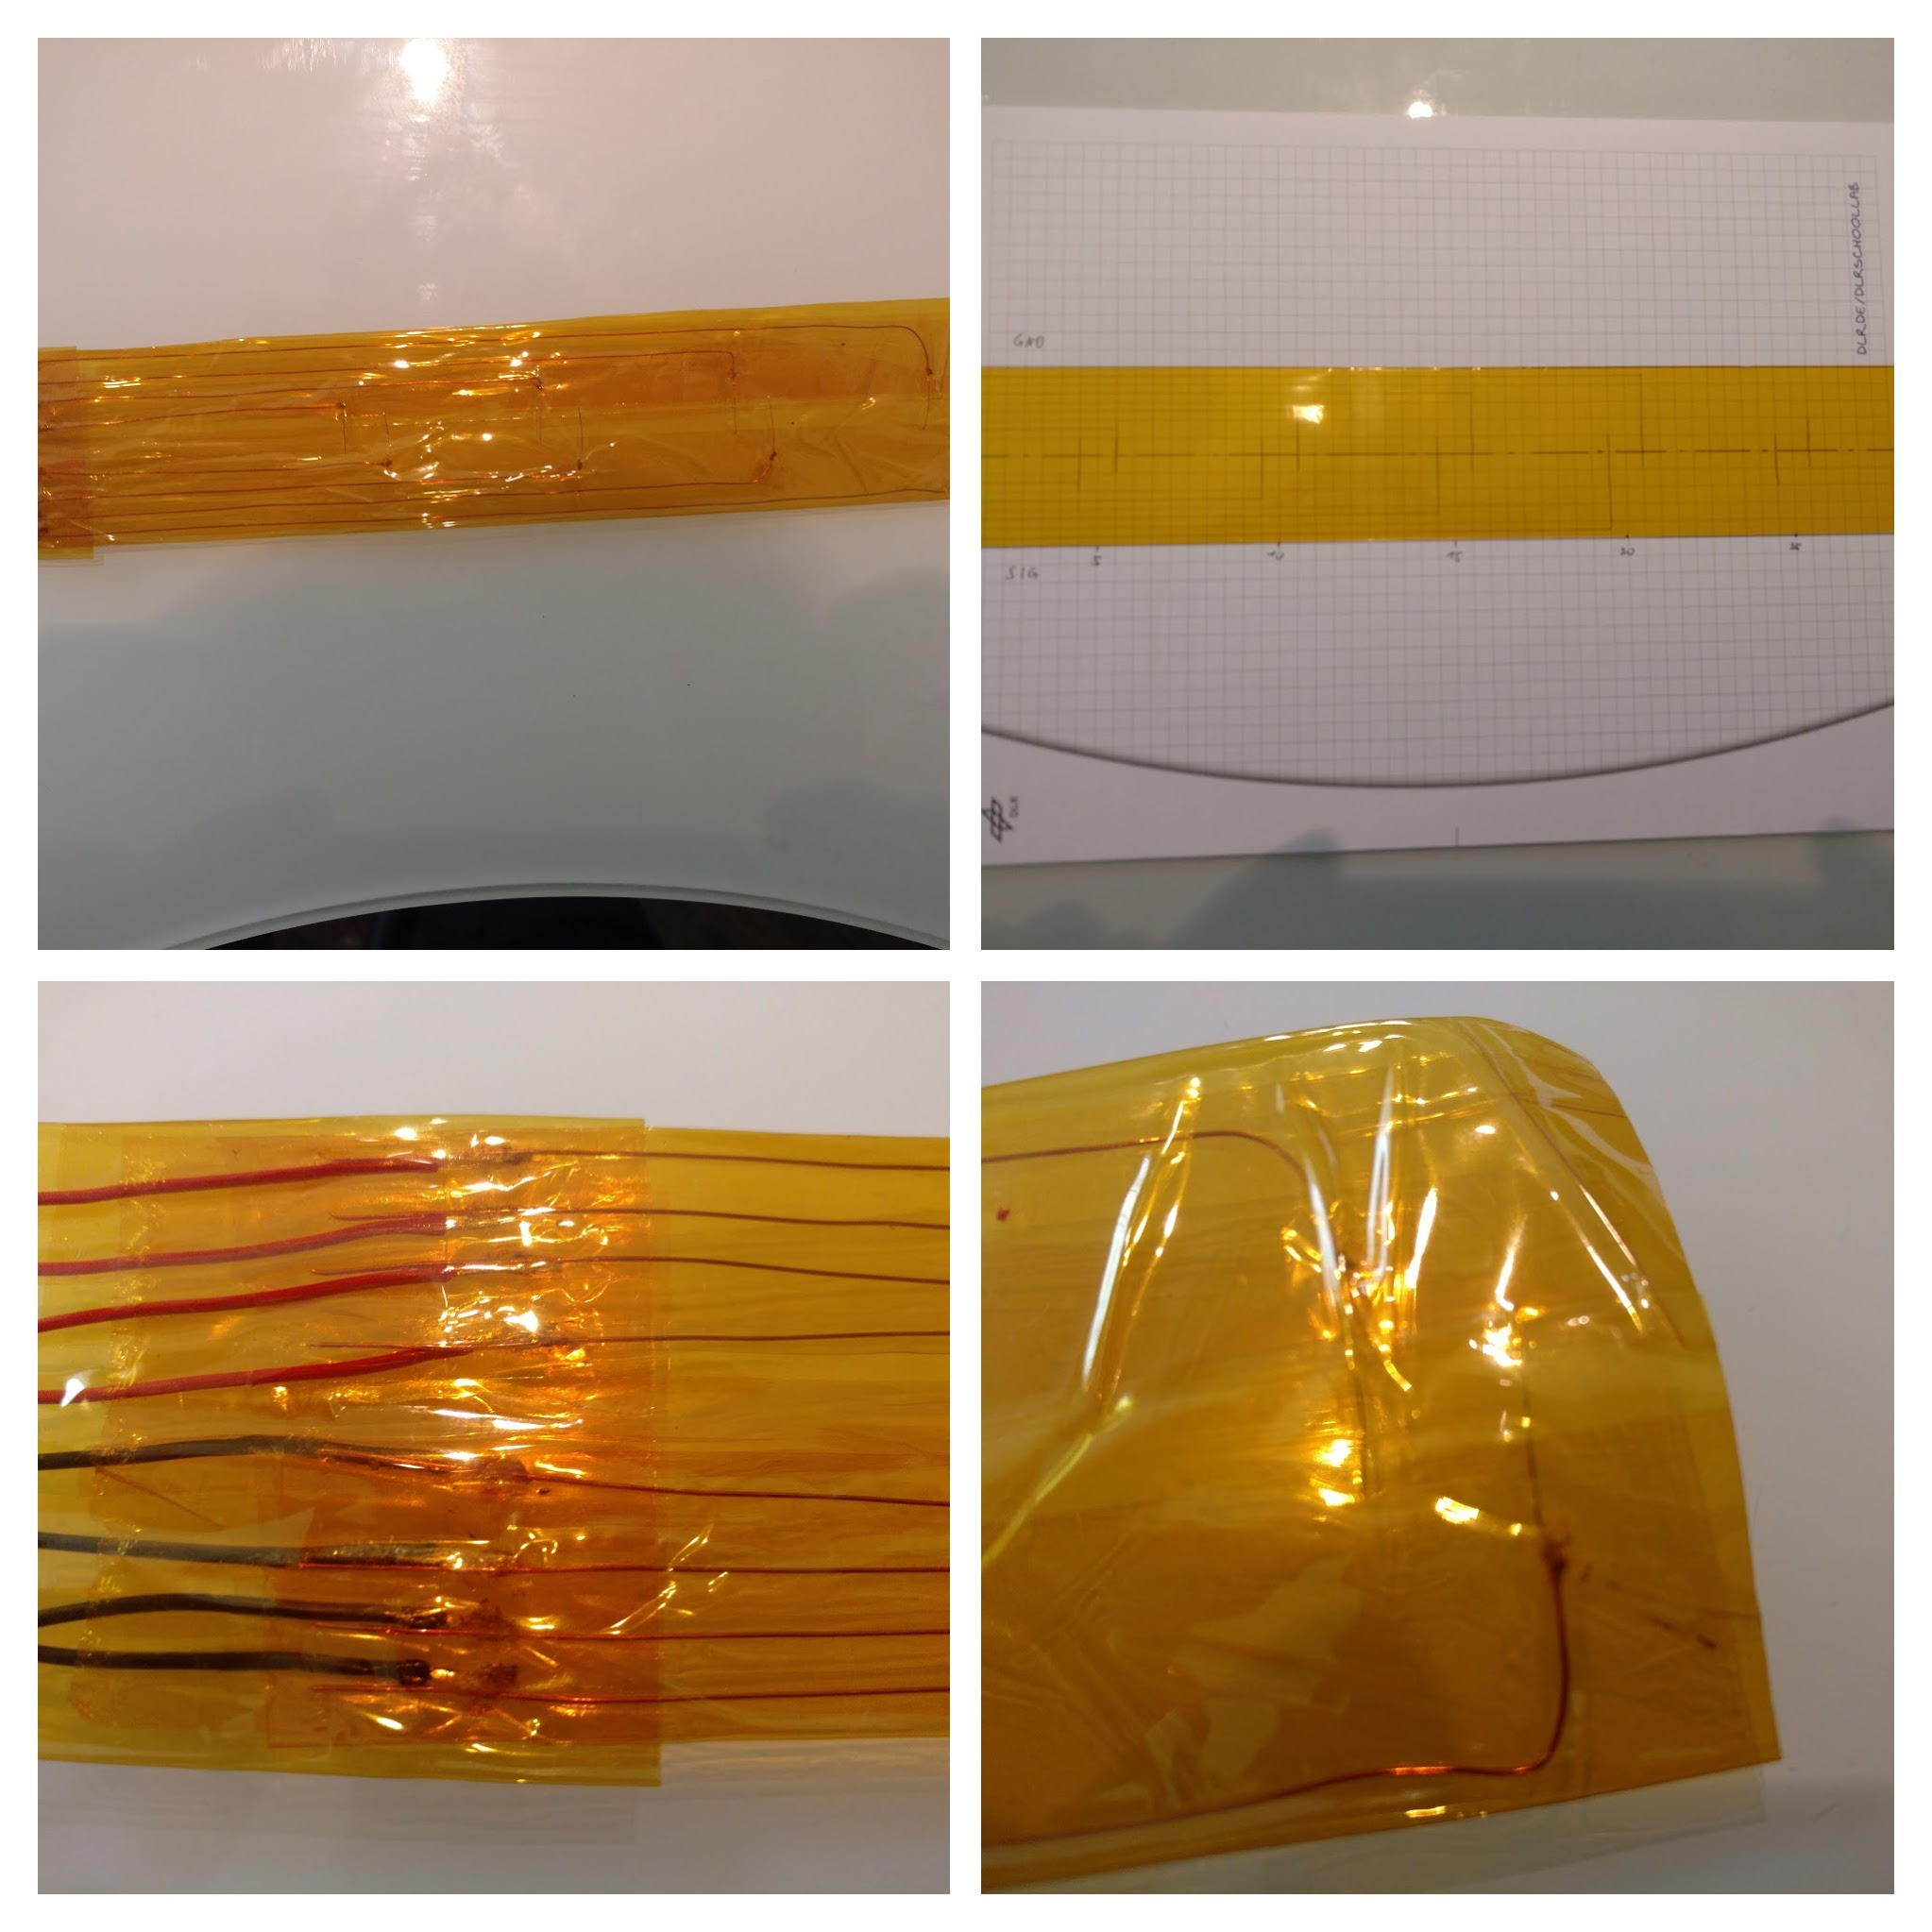
\includegraphics[width=\textwidth]{images/v2.jpg} 
		\caption{Handmade Sensor Strip}
		\label{fig:v2}
	\end{center}
\end{figure}

As an alternative to these handmade strips, industrially produced Flex-PCBs were identified. Flex-PCBs are flexible printed circuit boards that are very close to the handmade arrays described above. They also use Kapton as base, on which a copper coating gets applied and partially removed by etching to form the conducting paths. On top, another layer of Kapton is applied, with cutouts in the places where the copper is supposed to be exposed. The exposed copper is then plated with ENIG (Electroless nickel immersion gold) to protect the copper from oxidation and provide the landing pads for electrical components to be soldered on.

For our purpose those exposed and plated landing pads can be used as electrodes, being nicely embedded in a FlexPCB that also runs the wiring up to an interface from where cables can be run. Using the FlexPCB itself as cable is not viable due to the high cost per area.

The cables are soldered directly to the PCB and silicone is used to create a waterproof seal around the connection.

\begin{figure}
	\begin{center}
		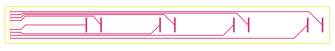
\includegraphics[width=\textwidth]{images/fpcbd.pdf} 
		\caption{Design of FlexPCB}
		\label{fig:fpcbd}
	\end{center}
\end{figure}

\section{Matrix Switches}

The matrix switches are an essential part of the system, enabling it use multiple sensors with a single MinieC Interface, thus lowering the cost per sensor. The part used is an ADG738 from Analog Devices. It is an 8-channel CMOS analog matrix switch controlled via a 3-wire serial interface. The following information is taken from the data sheet \cite{ms}.\\

Figure \ref{fig:ms} shows the functional block diagram. The switch has one drain pin (D) and 8 source pins (S1..S8). Despite the naming of drain and source, the internals provide simple switches between the drain and each source pin. The switches work in both directions without any restriction on the signal beyond a maximum current of \unit[120]{mA} that far exceeds our needs. By sending control commands via the 3-wire interface, each of the 8 internal switches can be turned on and off individually.\\

\begin{figure}
	\begin{center}
		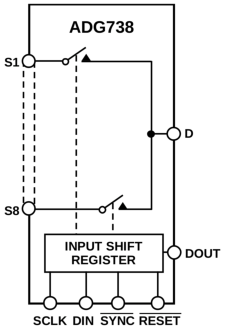
\includegraphics[width=0.3\textwidth]{images/ms.pdf} 
		\caption{Functional block diagram of ADG738}
		\label{fig:ms}
	\end{center}
\end{figure}

The example timing diagram \ref{fig:msc} describes the data transmission process. The microcontroller sends one byte of data to the matrix switch. Each of the 8 bits of this byte controls one switch. The first bit controls the first switch and so on. If the bit is 1, the switch is closed, if 0, the switch is open. To send the byte, first the synchronization pin (SYNC) has to be pulled low from it's usual high level. A clock signal is provided to the clock pin (SCLK). At each falling edge of the clock signal, the data input (DIN) is read - where high leads to a 1-bit and low to a zero-bit. After 8 cycles, SYNC is pulled high again marking the end of data transmission with a full byte transferred. After that, the switches immediately take their instructed states with switching times in the order of \unit[100]{ns}. In the example shown, the first switch is on, while all others are off.\\

\begin{figure}
	\begin{center}
	\tikzexternaldisable
		\begin{tikztimingtable}
  			SYNC   & H 32{L} H \\
  			SCLK   & C 16{2C} N(A1) C \\
  			DIN  	& 2{L} {2H} N(B1) 15{2L} \\
  			Data	& 2D{} 2D{1} 2D{} 2D{0} 2D{} 2D{0} 2D{} 2D{0} 2D{} 2D{0} 2D{} 2D{0} 2D{} 2D{0} 2D{} 2D{0} 2D{}\\
		\end{tikztimingtable}
		\caption{Timing diagram}
		\label{fig:msc}
	\end{center}
\end{figure}

Multiple matrix switches can be controlled at once by daisy-chaining the data output pin (DOUT) of the first device to DIN of the second one, and on so forth. Both SYNC and SCLK are connected to the same bus. This assures that all matrix switches are set in the same state and at the same time.

\section{MinieC Interface}

The sensor node logically consists of the signal generator and the signal reader, practically both parts are tightly integrated.

[Describe mini-eC-Interface]
[also where i.e. the change with the filter cap and the tests that surfaced the issue is described]

The mini-eC-Interface provides two channels to connect to the electrodes, but  multiple sensors should be driven by one interface. The method to this is called demultiplexing and the component able to this is the Matrix-Switch.
A Matrix-Switch is an electrical component containing a multitude of switches, where the switches can be electronically closed and opened from a controller. The Matrix-Switch chosen consists of 8 switches, where all switches have the same input, but separate outputs. Thus, they allow applying an input signal to different outputs. The input in our case is the signal and reference from the minie-eC-Interface, applied to 8 different electrode pairs making up the sensors. A separate Matrix-Switch is need for signal and reference.

\section{Microcontroller}

The Data Processing Unit has to be able to control the functions of the sensor nodes attached to it, read the data from them, log it and serve it to the user-interface. Typically, any micro-controller is is fit for those tasks. Micro-controllers usually are programmed in C or C++, however nowadays there are other options, too. One of those is Micropython, which is an implementation of the Python 3 programming language designed to run on micro-controllers. Python is a vastly easier language than C/C++, and this is especially true when the involved persons are not from a computer science or electrical engineering background, but i.e. mechanical engineering or other sciences. In those fields, Python is often familiar from usage for data processing and visualization. Using Micropython enables us to design a system where it is more likely that the people using it are able to understand the code, enabling them to improve it and adapt it to alternate use-cases.
It does however limit our choice of Hardware to supported platforms and it requires more powerful and thereby expensive micro-controllers. But as the system only requires one Data Processing unit to drive a very large amount of sensors, the added cost is relative and outweighed by the benefits of the better usability. While the factor of the expensive controllers to cheaper ones is about 10, the cost in the end is still only about \euro{7}.
For prototyping, a development board named "Espruino Pico" was chosen. It is a very small and simple board that provides the electrical boilerplate to use a micro-controller without needing to deal with the lowest level of electronics, like cleaning power supply, etc.

\section{User-Interface}